\section{Sensitivity of Internally Generated Field to Permeability of the Shield $B_0(\mu)$}

\subsection{Analytical Calculations in Spherical (and Cylindrical) Geometry}


%\begin{itemize}
%\item State basic physics of problem, define reaction factor, note
%  return flux through shield, etc.
%\item State formulae and results for reasonable parameters.
%\item Possibly one graph of $B_0(\mu)$ with both geometries.
%\end{itemize}

The presence of a coil inside the innermost passive shield turns the
shield into a return yoke and it is due to the penetration of the
magnetic field flux into the magnetic shield.  The ratio of the
magnetic field inside the coil in the presence of the magnetic shield
to that of the coil in free space is called the reaction
factor~\cite{bib:read_our_other_paper_for_some_references_that_say_this}.
Normally the reaction factor is larger than unity for spherical and
cylindrical geometries.  The key issue of interest for this work is
the dependence of the reaction factor on $\mu$.  This factor can be
calculated analytically for spherical and cylindrical
geometries~\cite{bib:bidinosti,bib:some_paper_from_1899}.  Although
the dependence of the reaction factor on $\mu$ is rather weak for
these geometries, the constraints on $B_0$ stability are very
stringent.  Thus a small change in the magnetic properties of the
innermost shield can result in an unacceptably large change in $B_0$.

%From Refs. \cite{bib:smythe, bib:ferraro} for a zonal surface current
%\begin{equation}
%\bold{F}=- \sum_{n=1} ^{\infty} \frac{C_n}{\ell} P^1 _n (u) \hat{\phi}
%\end{equation}
%bound on a sphere with radius $\ell$ the magnetic field at $r < \ell$ and $r>\ell$ is calculated.
%The case of an ideal spherical surface current ($n=1$) inside a spherical shell with inner radius $a$ and outer radius $b$ has been analytically calculated considering the following boundary conditions

%\begin{equation}
%\frac{1}{\mu_0} B_{\theta} (a^-) = \frac{1}{\mu} B_{\theta}(a^+)
%\end{equation}
%\begin{equation}
%\frac{1}{\mu}B_{\theta}(b^-)=\frac{1}{\mu_0}B_{\theta}(b^+).
%\end{equation}
%Fig. \ref{fig:Magnetic_Field} shows the magnetic field $B$ as a function of relative $\mu$ for $\ell=0.53$ m, $a=0.57$ m and a thickness of 1.5 mm for the shield which are comparable to the dimensions of the ILL nEDM experiment setup \cite{bib:baker, bib:knecht}.

Fig.~\ref{fig:Magnetic_Field} shows the central magnetic field $B$ as
a function of relative $\mu_r=\mu/\mu_0$ for coil radius 0.53~m inside
a magnetic shield with the inner radius of $0.57$~m and a thickness of
1.5~mm.  The dimensions have been selected to be comparable to the
dimensions of the ILL nEDM experiment
geometry~\cite{bib:baker,bib:knecht}.
\begin{figure}[h!]
\begin{center}
   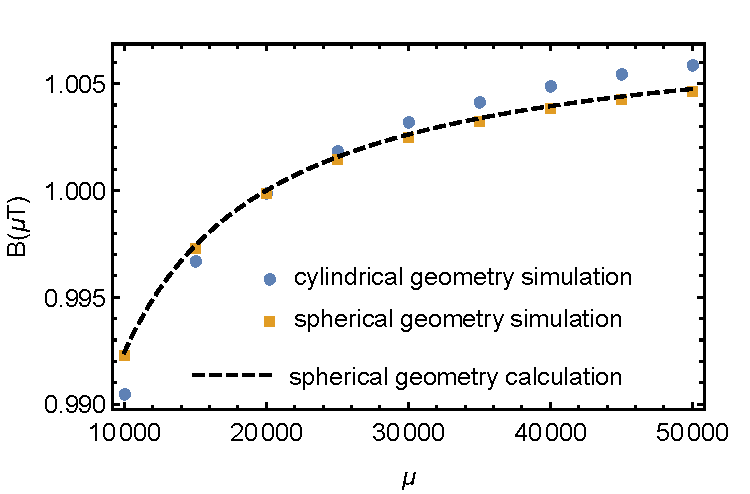
\includegraphics[width=0.6\textwidth]{femm_and_calcs.pdf}
    \caption{Magnetic field as a function of relative magnetic
      permeability $\mu_r$ for geometries similar to the ILL nEDM
      experiment.  The dashed line is for an ideal spherical surface
      current of radius 0.53~m inside a spherical shell of inner
      radius 0.57~m, thickness 1.5~mm.  Open and close circles are
      FEMM-based simulations of spherical and cylindrical geometries
      with similar dimensions, described in the text.  The coil
      currents have been arranged to give a $1~\mu$T field at the
      $\mu_r=20,000$ point.}
    \label{fig:Magnetic_Field}
    \end{center}
\end{figure} 
For a 10\% change in relative $\mu_r$ (from 20000 to 22000), the
magnetic field changes by 0.7~nT.



\subsection{Magnetostatic Simulation Results \label{sec:femm}}

Finite-element analysis simulations were conducted to analyze the
effect of discretizing the surface current, and to test the geometry
dependence of the sensitivity of the experiment to changes in $\mu$.
Two axially symmetric simulations were conducted using
FEMM~\cite{bib:femm}.  In the first simulation, the same spherical
geometry was used as for the analytical calculations.  However, the
surface current was discretized to 50 individual circular wires,
inscribed onto a sphere, and equally spaced vertically (i.e.~a
discrete cos$\theta$ coil).  A square sire profile of side length 1~mm
was used.  As shown in Fig.~\ref{fig:Magnetic_Field}, this simulation
gave good agreement with the analytical calculation.

As an example of one additional axially symmetric geometry, a solenoid
within a cylindrical shield was simulated, with equal coil spacings.
In the limit of infinite $\mu$, the image currents in the end caps of
the shield are an infinite series of coils, giving an ideal infinite
solenoid with a uniform field.  Again, fifty discrete coils were
simulated, where the spacing from an end coil to the inner face of the
shield end-cap being half the inter-coil spacing, as appropriate to
generate the correct image currents in the infinite $\mu$ limit. 

As shown in Fig.~\ref{fig:Magnetic_Field}, the slope of $B(\mu)$ is
somewhat steeper, and similar in magnitude to the spherical case.  We
therefore estimate that the scale of the sensitivity of a generic nEDM
experiment to global changes in the magnetic permeability is
$\frac{\mu}{B}\frac{dB}{d\mu}\sim 0.01$.

In the spherical case the reaction factor is 1.39, meaning that the
field generated by the spherical coil is amplified by this
multiplicative factor by the presence of the magnetic shield (flux
return).  In the cylindrical case the reaction factor is 1.35.  If the
reaction factor is closer to unity, the calculated
$\frac{\mu}{B}\frac{dB}{d\mu}$ will be smaller, and the EDM experiment
less sensitive to changes in $\mu$.  The results in the two geometries
show that there is also a weaker geometry dependence to this
statement.


%\begin{itemize}
%\item I think it would be easy to provide results in axisymmetric
%  geometries from FEMM.
%\item If any result is available from OPERA, it could be included here.
%\item Results should be for a restricted set of possible nEDM coils.
%\item quote reaction factors?
%\item One graph?  % probably the same graph as above
%\end{itemize}

\subsubsection{Field within the passive flux return for EDM experiments}

For a high-$\mu$ innermost shield, the magnetic field lines emanating
from the coil all return through the shield.  This principle can be
used to estimate the magnetic field internal to the material, and in
our studies gave good agreement with FEA-based simulations.  For the
cylindrical geometry described in Sec.~\ref{sec:femm}, the $B$ field
is largest in the side walls of the cylindrical flux return, attaining
a maximum value of 170~$\mu$T.  For $\mu_r$=20,000 (a typical
realistic value for the DC value of $\mu_r$ in these shields), the $H$
field is 0.007~A/m.  These values are weakly dependent on $\mu_r$.
They set a scale for the values of $B$ and $H$ which we sought to
replicate in our experiments reported in Section~\ref{sec:tdep}.

% Jeff and Taraneh to do: confirm by checking against FEMM.  Possibly
% add more numbers for spherical geometry.


\subsection{Self-Shielded Coils}

A way to decouple the internal coil from the magnetic shield is to
design a self-shielded
coil~\cite{bib:cpviolwithoutstrangeness,bib:someotherselfshieldedcoilpapers}.
In self-shielded coils, the return flux is provided by a second larger
coil, rather than through the permeable material of the magnetic
shield.  In a perfect self-shielded coil, the field at the position of
the magnetic shield would be zero, resulting in a reaction factor that
is identically unity.

Such coils would completely decouple the properties of the magnetic
shield from the homogeneity and stability of the coil itself.  Changes
in $\mu$ of the shield material would then have no impact on the nEDM
experiment.  Coils incorporating self-shielding in their design are
therefore an attractive option for nEDM
experiments~\cite{bib:cpviolwithoutstrangeness}.


%\begin{itemize}
%\item Explain principle (reaction factor = 1, or no field at shield so
%  no return flux)
%\item Simple analytic results - reaction factor is identically unity.
%\item FEMM/OPERA - demonstrate that sensitivity is reduced by factor
%  of XX for simple geometry.
%\item One graph, or include on previous graph?
%\end{itemize}

\subsection{Summary of $B_0(\mu)$}

For shield-coupled coils, the magnetic field in the region interior to
the coil is coupled to the properties of the magnetic shell which is
caused by the penetration of the magnetic field flux into the shell
material. In a typical nEDM experiment, the sensitivity of the
internal magnetic field to changes in $\mu$ is
$\frac{\mu}{B}\frac{dB}{d\mu}\sim 0.01$.  The coupling can be reduced
considerably by using a self-shielded coil design, which does not
couple strongly to the innermost magnetic shield.

The field generated in the innermost magnetic shield by a
shield-coupled coil is typically $B=170~\mu$T, corresponding to
$H=0.007$~A/m.  The field in the nEDM measurement volume, as well as
in the magnetic shield, must be stable for periods of typically
hundreds of seconds (corresponding to frequencies $<<0.01$~Hz).  This
sets the relevant measurement scales for magnetic properties that
would be most relevant to nEDM experiment.